\chapter{Avaliação Semi-Automática de Questões Discursivas}\label{cap3}
Nesse capítulo, apresentamos a abordagem do sistema na correção de atividades discursivas. Definimos então a extração de informações dos AVA, a padronização da escrita, o reconhecimento de padrões de resposta, a avaliação semiautomática de questões discursivas e o retorno de resultados aos participantes da disciplina para após compararmos os efeitos da seleção de características isoladamente. Dessa forma, com a inclusão do mapa de características no sistema, podemos analisar a influência da redução de dimensionalidade na melhoria das formas de classificação e visualização da informação para cada atividade.

\section{Coleta de Dados}

Certas ferramentas de mineração de dados auxiliam a aquisição de conhecimento em inúmeros procedimentos do cotidiano. Entre eles, a educação não é uma exceção, apesar de ser pequena a aplicação nas salas de aula tradicionais. Com o emprego dos Ambientes Virtuais de Aprendizagem e a popularização dos Cursos Online Abertos e em Massa - MOOC's a quantidade de dados produzidos e a necessidade de apoio aos profissionais dessa área se tornam cada vez maiores. Porém, para processamento desses dados é necessária a extração das plataformas de ensino e o transporte para servidores pré-configurados com os Sistemas de Apoio - SA.

\begin{comment}
As pesquisas em Mineração de Dados Educacionais - EDM gradativamente se adéquam às grandes demandas provenientes das ferramentas que suportam a construção e desenvolvimento dos MOOC's. Para atender a produção cotidiana de dados e apoiar os instrutores das disciplinas busca-se aderir à tecnologia na aquisição de informações de forma semelhante à um especialista. Porém, para processamento desses dados é necessário extraí-las das plataformas de ensino e transportá-las para servidores pré-configurados com os Sistemas de Apoio - SA, garantindo atender seus requisitos e os isolando de qualquer possível interferência.
\end{comment}

Segundo o site oficial com estatísticas sobre o Moodle\footnote{Estatísticas do uso do Moodle. Disponível em: https://moodle.net/stats/}, atualmente são 72 mil sistemas cadastrados em 232 países do mundo. Com 95 milhões de usuários, esse AVA é um grande exemplo de produtividade acadêmica que certamente têm alto custo aos profissionais de ensino que, individualmente, avaliam todos os alunos. Com uma estrutura de coleta de informações, tornamos possível o processamento das bases de dados para apoio ao processo de ensino-aprendizagem. Com a extração desses dados, beneficiamos os participantes dos cursos \textit{online} incentivando a discussão de resultados, elaborando relatórios para manter o professor atento ao andamento do curso.

Para habilitar o apoio ao tutor, um Sistema de Transferência de Dados - STD interage diretamente com o banco de dados da plataforma de ensino para coletar os documentos produzidos pelos estudantes. Por meio do \textit{web service}, o STD, interliga ambientes virtuais e o servidor de processamento. Cada SA desenvolvido torna-se um serviço acionado pelo professor na configuração da tarefa, recebendo resultados diretamente na plataforma. Essa arquitetura é apresentada na Figura \ref{fig-architecture} de forma a manter os serviços em alta disponibilidade para todos os AVA.

\begin{figure}[ht]
\centering
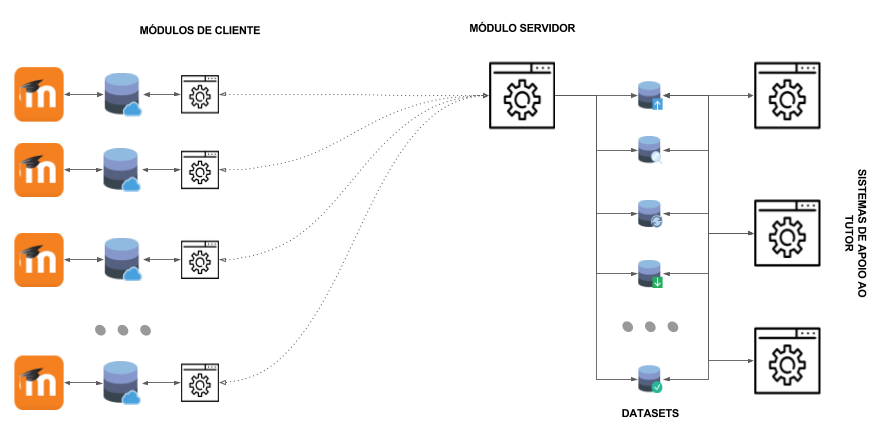
\includegraphics[width=.9\textwidth]{img/plugin_moodle.png}
\caption{Arquitetura do sistema de extração de dados dos AVA.}
\label{fig-architecture}
\end{figure}

Como pode ser visto na Figura \ref{fig-architecture}, a interação dos dois tipos de servidores ocorre através do \textit{web service} do Sistema de Transferência de Dados. Nessa arquitetura, os dados são extraídos dos Ambientes Virtuais de Aprendizagem para processamento nos Sistemas de Apoio. Cada \textit{software} é descrito em detalhes à seguir.

\subsection{Ambientes Virtuais de Aprendizagem - AVA}
Os AVA's são ambientes de suporte ao ensino que modelam as informações para auxiliar na evolução da disciplina. O seu uso permite a organização de atividades e materiais didáticos para os participantes terem amplo acesso ao conteúdo. A alta disponibilidade atrelada a esses sistemas amplia o tempo de disciplina para além das aulas presenciais viabilizando o EaD e a extensão dos planos de estudo.

Além de impactar diretamente na metodologia de ensino e aprendizagem, o uso dos AVA é muito relevante para coleta de dados educacionais. A sua organização deixa à disposição todos os dados, permitindo a criação de ferramentas que observem cada tarefa, nota, aluno ou professor. Com esse tipo de conhecimento, é possível compreender as avaliações, dificuldades e recomendações dos usuários para melhoria de desempenho.

\subsection{Sistema de Transferência de Dados - STD}
Os sistemas de transferência de dados são dois módulos integrados aos servidores que conectam os SA aos AVA. As ferramentas interagem com o servidor para transformar informações em arquivos estruturados a serem transportados através de \textit{web services}. Basicamente, a colaboração entre tais sistemas é o que permite a fluidez das informações em trânsito nos servidores.

Nessa arquitetura, o primeiro modulo é integrado ao AVA e aguarda solicitações de coleta e inclusão de dados. As informações da tarefa, notas, submissões e \textit{feedbacks} são utilizados para obter o conhecimento necessário para as técnicas de mineração de dados acopladas no segundo módulo. Porém, no segundo módulo, os dados coletados são interpretados por um sistema específico já conhecido e designado pelo professor. O SA, com a requisição, observa o comportamento dos usuários e corresponde conforme suas ações.

Dessa forma, os módulos em determinados espaços de tempo interagem para passagem de informações e processamento sob demanda. Os dados são atualizados a cada \textit{download} e os resultados são diretamente enviados às respectivas plataformas de ensino. No AVA, todos os participantes dos cursos recebem simultaneamente os resultados de modo transparente enquanto o tutor pode inserir suas próprias notas e/ou \textit{feedbacks} a qualquer momento.

\subsection{Sistema de Apoio - SA}
Os Sistemas de Apoio - SA realizam toda a parte de processamento e atendimento de necessidades específicas aos usuários dos AVA. Com a coleta de dados sendo realizada para todos os ambientes virtuais cadastrados, as bases de dados são processadas pelas ferramentas indicadas pelo professor durante a elaboração da tarefa. Nessa configuração é designado o sistema para apresentar detalhes relevantes sobre a base de dados de forma a suportar os métodos de ensino e aprendizado.

Esse tipo de ferramenta têm como objetivo realizar a mineração de dados para informar aos participantes sobre o andamento do curso. Com relatórios e conhecimentos em torno da atividade ficam evidentes os critérios de avaliação para recuperação de conteúdo, verificação colaborativa e recomendações de aprendizado.

O SA proposto nesse trabalho é o mapa de características, descrito detalhadamente no Capítulo \ref{cap4}, para redução de dimensionalidade e representação dos dados. Essa ferramenta, além de ser um método de visualização dos resultados ainda facilita os processamentos eliminando características irrelevantes. Tais características, diretamente extraídas da escrita dos alunos, são as informações que o sistema mantém pela ocorrência na avaliação do professor. Sendo automático, a melhoria com visualização dos resultados proporciona aos usuários a discussão colaborativa e classificações mais adequadas.

\section{Modelo Vetorial}\label{modelo_vetorial}
Após a coleta e o armazenamento de resultados o sistema controla a aquisição de informações sobre a base de dados. Para isso é utilizado o modelo vetorial descrito por \cite{salton1975}. Como forma de interpretação computacional de documentos, o tipo de vetorização adotado ocorre através da frequência dos termos indexados à partir dos textos, ou \textit{Term Frequency - TF} em inglês. Esse modelo se baseia na técnica de processamento de textos ``\textit{bag of words}'' onde cada índice é associado a um termo distinto encontrado no conjunto de documentos.

No modelo vetorial, cada documento \textit{d} de um conjunto de documentos $ D = \{ d_{1} , d_{2} , d_{3} , \dots , d_{|D|} \} $ é representado como um vetor de termos \textit{t}. Durante a vetorização. é verificada a frequência de ocorrência (TF) de cada um dos \textit{t} termos em cada documento \textit{d} em \textit{|D|}, sendo \textit{|D|} o total de documentos desse conjunto. Para cada \textit{d}, portanto, é computada a frequência individual dos $ t = \{ t_{1}, t_{2}, t_{3}, \dots , t_{k} \} $ termos que existem na base de dados, sendo \textit{k} o número de termos distintos encontrados na coleção. Assim, cada documento \textit{d} é representado como um vetor com as frequências individuais \textit{n} de cada um dos \textit{k} termos distintos, como o exemplo visto na Equação \ref{modelo-vetorial}.
\begin{equation*}
d_{0} = \{ n_{t_{1}} , n_{t_{2}} , n_{t_{3}} , \dots , n_{t_{k}} \}
\end{equation*}
\begin{equation*}
d_{1} = \{ n_{t_{1}} , n_{t_{2}} , n_{t_{3}} , \dots , n_{t_{k}} \}
\end{equation*}
\[\vdots \]
\begin{equation}
d_{|D|} = \{ n_{t_{1}} , n_{t_{2}} , n_{t_{3}} , \dots , n_{t_{k}} \}
\label{modelo-vetorial}
\end{equation}

Na forma numérica, o documento passa a ser interpretado no espaço vetorial. Com os valores \textit{n} de cada característica \textit{t} no determinado temos $ n_{t_{d}}$, ou seja, o valor da frequência desse termo em um determinado documento \textit{d}. Após a transformação, os vetores são comparados segundo a ocorrência dos seus termos, a similaridade dos vetores e a correlação entre as frequências.

Outros modelos com a inclusão de ponderações sobre as características são utilizados para estudo da distribuição dos termos entre documentos ou classes. O método mais tradicional \textit{Inverse Document Frequency - IDF} \cite{baeza2011} é um exemplo disso, onde termos que ocorrem em vários documentos recebem peso menor do que termos raros, o que prioriza os que possivelmente são diferenciais entre classes. Neste trabalho porém, foi usada a distribuição original (TF) sem pesos, avaliando a redução de dimensionalidade diretamente sobre a classificação do especialista. Estudos com as várias ponderações devem ser feitas para uma análise da distribuição de cada característica, vendo a adequação dos termos com o interesse desse trabalho, como as esperadas pelo usuário através de sua avaliação.

\subsection{Similaridade de Cosseno} \label{similaridade}
Para as análises computacionais, a similaridade de cosseno permite parear vetores de documentos para análise estatística, reconhecimento de padrões e definição de agrupamentos. O cálculo é dado em pares de documentos para compará-los através do conteúdo normalizado. Então, a similaridade adotada é um modelo matemático que quantifica a distância entre documentos no espaço vetorial.

A distância de cosseno, segundo \cite{baeza2011}, é a métrica mais usual para a comparação entre documentos textuais. Nessa análise de similaridade, um valor entre 0 e 1 representa o quanto pares de documentos são idênticos, onde os exatamente iguais têm similaridade 0 e, por consequência, os completamente dissimilares 1. A similaridade de cosseno é representada pela Equação \ref{eq-cosseno}.

\begin{equation}
Sim_{cos}(d_{i},d_{j}) = \frac{d_{i}.d_{j}}{||d_{i}.d_{j}||}
\label{eq-cosseno}
\end{equation}

Na Equação de distância de cosseno \ref{eq-dis-cosseno}, é uma transformação do resultado da razão entre a multiplicação e a intercessão do par $(d_{i},d_{j})$, dado pela similaridade, (Equação  \ref{eq-cosseno}) em uma métrica de distância. A diferença está na inversão dos valores com menores para vetores equivalentes e maiores para distintos. Na métrica de distância valores também estão entre 0 e 1. Porém, quanto mais próximos de 0 maior a equivalência dos documentos, sendo zero retornado para vetores de mesma norma. Em contrapartida, valores próximos à 1 representam vetores distintos.
\begin{equation}
D_{cosseno_{(d_{i}, d_{j})}} = 1 - Sim_{cos}(d_{i},d_{j})
\label{eq-dis-cosseno}
\end{equation}

\subsection{Pré-Processamento}
A padronização dos documentos é um procedimento comum para a extração de informações e redução de dimensionalidade. Para isso, algumas análises por NLP do conteúdo visam manter termos equivalentes e correlacionados, removendo palavras que não adicionam informações relevantes ao texto. A padronização de escrita utilizada pelo sistema é dada pela remoção de \textit{stopwords}, \textit{stemming} e tokenização, descritas individualmente abaixo.

\subsubsection{Remoção de {\it Stopwords}}
A remoção de \textit{stopwords} \cite{manning1999} foi utilizada para extrair da avaliação e recuperação de informação as palavras que possivelmente nada adicionam ao contexto. Nesse processo todas as palavras de uma lista pré-definida são excluídas do texto antes da vetorização. As palavras excluídas, geralmente, são conectivos textuais já conhecidos da linguagem. Esses termos, durante a interpretação computacional, não influenciam nas informações passadas pelo interlocutor e são removidos para estudo do conteúdo.

As listas de \textit{stopwords} para inglês e português são apresentadas nas Tabelas \ref{tab-stopwords-en} e \ref{tab-stopwords-pt}.

\subsubsection{{\it Stemming}}
Stemmização é outra importante padronização do conjunto de documentos, que consiste na radicalização de todas as ocorrências das palavras através da remoção de afixos \cite{weiss2010}. Marcantes na língua portuguesa, com várias sintaxes e modificadores, esse processo remove prefixos e sufixos para destacar apenas o morfema básico nos grupos textuais e nas referências de avaliação.

Com a aplicação desse método, palavras em pessoa, número ou tempo diferentes são normalizadas para um mesmo radical. Dessa forma, espera-se que uma frase escrita em todas as possíveis conjugações sejam interpretadas de forma equivalente pelo sistema, apesar da perda de informação.

\subsubsection{Tokenização}
A tokenização é a separação das palavras dentro de uma frase para posterior vetorização \cite{manning1999}, sendo a etapa responsável pela inclusão de métodos de tratamento do conteúdo. Nessa etapa os dados indesejáveis como as \textit{stopwords}, acentuação e a pontuação são eliminados.

Porém durante a tokenização, para identificar conexões textuais as palavras foram extraídas em faixas de \textit{n-grams}. Os \textit{n-grams} são a quantidade de palavras analisadas em uma distância \textit{n}. Assim, dentro de cada documento \textit{d} é verificada a frequência de grupos de palavras de \textit{n} distância. Caso seja 1 (\textit{unigram}), a resultante da vetorização será igual a gerada por TF. 

Nesse caso, especificamente, foram coletados de 1 a 3-\textit{grams} (\textit{unigrams}, \textit{bigrams} e \textit{trigrams}). Por exemplo, se temos uma frase formada por seis termos com índices $ \{ t_{45} , t_{32} , t_{123} , t_{1024} , t_{256} , t_{13} \} $, essa coleta é dada da seguinte forma:

%\begin{comment}
\newcommand{\sep}{\hspace*{0.3em}}

\noindent1-\textit{gram}:
   $ \fbox{ \{t_{45}\} \sep \{t_{32}\} \sep \{t_{123}\} \sep \{t_{1024}\} \sep \{t_{256}\} \sep \{t_{13}\} } $
   
\noindent2-\textit{grams}:
   $ \fbox{ \{t_{45}; t_{32}\} \sep \{t_{32}; t_{123}\} \sep \{t_{123}; t_{1024}\} \sep \{t_{1024}; t_{256}\} \sep \{t_{256}; t_{13}\} }$
   
\noindent3-\textit{grams}:
    $ \fbox{ \{t_{45}; t_{32}; t_{123}\} \sep \{t_{32}; t_{123}; t_{1024}\} \sep \{t_{123} t_{1024}; t_{256}\} \sep \{t_{1024}; t_{256}; t_{13}\} } $

%\end{comment}

Esse modelo de extração apresenta os grupos de termos como os destacados acima, onde são organizados conjuntos conforme a ocorrência por vizinhança. Simultaneamente, com a definição das características textuais no conjunto \textit{D}, é realizada a contagem da frequência para cada documento \textit{d}. Desse modo, torna-se possível a realização das comparações entre os documentos através da Equações \ref{eq-cosseno} e \ref{eq-dis-cosseno} para análise por pares.

\section{Algoritmo Genético}
Aplicado na seleção de características para redução de dimensionalidade, o Algoritmo Genético - GA \cite{haupt2004} é inspirado na teoria da evolução darwiniana. Sua otimização funciona através de combinações vetoriais para a melhoria das soluções candidatas com avaliação qualitativa através da função de \textit{fitness}. Cada solução candidata remete à um cromossomo, sendo conjuntos de valores denominados genes. Cada um passa pelo processo de seleção, \textit{crossover} e mutação. Na seleção é definido o par da população que realizará a combinação. O \textit{crossover} é a função responsável pela combinação do par de cromossomos candidatos selecionados para criação de novos indivíduos. A etapa de mutação altera os dados (ou genes) para adicionar variações genéticas na população.

Para o GA, é necessário criar uma população que será a distribuição de valores disponíveis para combinação. A otimização é ciclica, ou seja, ocorre com um dado número de iterações. Para cada ciclo completo de etapas, chamado de gerações, o melhor item resultante é comparado com os vetores populacionais.  Se esse indivíduo de melhor \textit{fitness} gerado tiver valor superior ao pior elemento existente da população ele o substitui.

Aplicado à seleção de características \cite{raymer2000}, os vetores das \textit{k} características são combinadas para eliminação de informações conforme a otimização da métrica. No caso do mapa de características, foi aplicada uma razão da quantidade de termos selecionados pela similaridade interna da classe. Espera-se, portanto, reduzir a quantidade de termos do conjunto enquanto se amplia a similaridade média do grupo, tornando-o mais denso. Com maior densidade, os documentos são sumarizados e espera-se que representem a essencia do conjunto de informações.

\section{Aprendizado Semi-Supervisionado}
Na inteligência artificial, sistemas são classificados quanto ao seu modelo de aprendizado de forma dependente ou independente do especialista. Nos sistemas supervisionados o especialista treina o algoritmo com uma quantidade de dados para atuação desse na tarefa. Esse modelo criado direciona a qualidade dos resultados através da interpretação e completude dos padrões nos exemplos apresentados. Por outro lado, os não-supervisionados são independentes da classificação de um especialista para descoberta de padrões e a aquisição de conhecimento. O paradigma desse modelo é exploratório, ou seja, o próprio sistema busca nos dados as informações para a especialização do trabalho.

Para a avaliação de questões discursivas, a definição do critério de correção é fundamentada na busca conhecimento de um especialista. Nesse caso, o conhecimento pode ser a avaliação do professor, porém atentando-se à redução do esforço do humano. Pensando na sobrecarga desse profissional utilizamos da supervisão humana apenas durante a avaliação dos padrões identificados automaticamente. Dessa forma, diferentemente dos dois modelos clássicos de aprendizado, os exemplos requisitados para treinamento são selecionados pelo próprio sistema. Nesse sistema, utilizamos do aprendizado semi-supervisionado, onde através de uma combinação de clusterização (não-supervisionado) e classificação (supervisionado), buscamos identificar previamente os requisitos da avaliação. Nesse formato, o fator de avaliação humana é um passo intermediário entre a descoberta de padrões e a obtenção dos resultados pós-classificação.

\subsection{Combinando Clusterização e Classificação}
Para definição dos padrões para os métodos de avaliação analisamos a distribuição espacial dos agrupamentos. Os grupos de documentos foram formados conforme os resultados da clusterização com distância de cosseno (Equação \ref{eq-dis-cosseno}). Esse processo utiliza o CLUTO \footnote{http://glaros.dtc.umn.edu/gkhome/views/cluto} \cite{karypis2002} para testes do número de grupos visando reduzir a taxa de sobreposição, ou \textit{ovelapping} em inglês. Essa taxa de \textit{ovelapping} é obtida através da Equação \ref{eq-silhouette} do \textit{silhoutte score} \cite{rousseeuw1987}. Os testes de número ideal de grupos se dão pela execução do sistema para todas possibilidades de 3 até \textit{c} de grupos, sendo \textit{c} o máximo definido por $ \sqrt{\frac{|D|}{2}} \times{2} $. O agrupamento de melhor \textit{silhoutte score} é utilizado como ideal.

\begin{equation}
s_{cluster_{c}} = \frac{b - a}{max(a, b)}
\label{eq-silhouette}
\end{equation}

No coeficiente \textit{silhouette} para um determinado número de agrupamentos $ s_{cluster_{c}} $ , a variável \textit{a} refere-se à distância intra-\textit{cluster}, enquanto \textit{b} à média de distância de cada amostra até o \textit{cluster} mais próximo. Essa métrica retorna valores entre -1 e 1, sendo que os valores negativos representam arranjos ruins de amostras e os positivos \textit{clusters} bem definidos. Valores próximos à 0 representam \textit{clusters} em \textit{ovelapping}.

Essa métrica foi utilizada justamente na tentativa de contornar altas taxas de \textit{ovelapping} esperando o aumento da densidade dos agrupamentos. Com grupos bem selecionados nessa etapa, o treinamento do algoritmo deve ser mais representativo para a diversidade textual das submissões, permitindo a análise de \textit{clusters} mais objetiva para a classificação.

\subsection{Identificação de Treino e Teste}
Na clusterização resultante, com base na análise intra-\textit{cluster} estudada por \citeonline{oliveira2014}, escolhemos itens que definam as melhores características para avaliação. Selecionamos para cada agrupamento os itens mais similares, mais dissimilares e de maior e menor norma para a correção do professor. Os de maior similaridade tendem à referenciar conteúdos equivalentes para um possível grupo de nota. Os mais dissimilares, ao contrário, representam as ideias divergentes do mesmo grupo. Os vetores de maior e menor norma estabelecem, respectivamente, os conteúdos extensos e resumidos associados para a avaliação. A extensão dos documentos é aplicada essencialmente no cálculo de representatividade das características, influenciando diretamente no método avaliativo.

Após a avaliação dos itens de treinamento pelo professor, são selecionadas as características, definindo conjuntos mínimos para cada nota. Então, cada nota atribuida pelo professor torna-se um rótulo (classe) para as amostras, desconsiderando os grupos obtidos na etapa de clusterização. Esse processo de seleção com o mapa de características é descrito detalhadamente no Capítulo \ref{cap4}.

Com os conceitos mínimos por classe, o número de características total diminui consideravelmente reduzindo o esforço de interpretação e correção feito pelo algoritmo. Dois classificadores são utilizados para o processo de avaliação o \textit{k-vizinhos mais próximos}- \textit{K}-NN e o classificador baseado em centroide - CBC.
 
\subsection{{\it K-Nearest Neighbors - K-NN}} \label{knn}
O algoritmo \textit{K}-NN é um classificador escolhido pela classificação por associação aos padrões de treinamento. Nesse algoritmo, o modelo é criado através dos dados de treinamento, onde as características dos \textit{k} vizinhos mais próximos definem a classe de cada item de teste \cite{baeza2011}. A comparação é realizada pela distância de cosseno entre pares. Esse classificador tende a criar zonas de influência sinuosas no espaço vetorial através dos K termos de menor distância para o elemento sem classificação. Para $ K = 1 $, como nesse caso, o documento recebe o rótulo do item de treino mais similar.

Nesse problema, o \textit{K-NN} com $ K = 1 $ é utilizado por conta das atividades com poucas respostas e as notas raras no conjunto de avaliações. O algoritmo, portanto, mantém a distribuição da base de treino classificando os demais conforme documentos análogos (padrões conhecidos).

\subsection{{\it Centroid Based Classifier - CBC}} \label{cbc}
A classificação baseada em centroide, também conhecida por \textit{Rocchio}, é uma forma de extração de modelo de classes baseada no ponto médio (centroide) \cite{baeza2011}. Para cada classe é calculada a média entre os itens e, para cada elemento sem classificação, é atribuída a classe do centroide mais próximo. Assim, cada classe é representada pelo item médio na etapa de classificação.

Nesse caso, a escolha do \textit{Centroid Based Classifier} - CBC da-se pela recomposição de \textit{agrupamentos} por classes tal como os formados na etapa de \textit{clustering}. Para esse classificador são criadas zonas de influência por centroide no espaço vetorial o que o torna menos suscetível à \textit{outliers} do que o \textit{K-NN}.

\subsection{Métricas de Avaliação} \label{metricas}
Para avaliar a qualidade das classificações do sistema (Capítulo \ref{cap5}), utilizamos algumas métricas para validação dos resultados \cite{cohen1995}. Nos métodos onde o sistema identifica que o treinamento é dado em notas contínuas, o sistema compara as notas com o especialista através do Erro Médio Absoluto - MAE, do Erro Quadrático Médio - MSE e/ou do Desvio Padrão do Erro - SEM.

O Erro Médio Absoluto - MAE (\textit{Mean Absolute Error}), apresentado na Equação \ref{eq-mae}, calcula a diferença média relativa às predições do classificador ou regressor quando comparados com os valores reais atribuídos pelo especialista.

\begin{equation}
MAE_(y_{real},y_{pred}) = \frac{1}{n_{amostras}}\sum_{i=0}^{n_{amostras}-1}|y_{i_{real}}-y_{i_{pred}}|
\label{eq-mae}
\end{equation}

O Erro Quadrático Médio - MSE \textit{Mean Squared Error}), apresentado na Equação \ref{eq-mse}, calcula o quadrado da diferença média para as predições do sistema se comparados com os valores atribuídos pelo avaliador humano. A diferença entre o MSE e o MAE está na penalização de erros maiores causados principalmente pelos \textit{outliers}.

\begin{equation}
MSE_(y_{real},y_{pred}) = \frac{1}{n_{amostras}}\sum_{i=0}^{n_{amostras}-1}{(y_{i_{real}}-y_{i_{pred}})}^{2}
\label{eq-mse}
\end{equation}

O Desvio Padão do Erro - SEM \textit{Standard Error of the Mean}), apresentado na Equação \ref{eq-mse}, calcula o desvio das amostras da média (erro) para os valores preditos pelo sistema comparado-os com os valores atribuídos pelo avaliador humano. O valor retornado pode ser associado às métricas de erro para análise da distribuição do erro conforme os valores médios obtidos através do MAE.

\begin{equation}
SEM_(y_{real},y_{pred}) = \frac{\sigma}{\sqrt[]{n_{amostras}}}
\label{eq-sem}
\end{equation}

Os problemas de classificação são analisados qualitativamente com as métricas de \textit{precision}, \textit{recall}, \textit{accuracy} e f1, detalhadas abaixo.

A acurácia, ou \textit{accuracy}, dada pela Equação \ref{eq-acc}, avalia a proximidade das notas atribuídas para os valores conhecidos, resultando no erro. O resultado desse cálculo é o percentual dos itens avaliados de forma equivalente.
\begin{equation}
Accuracy_(y_{real},y_{pred}) = \frac{1}{n_{amostras}}\sum_{i=0}^{n_{amostras}-1}{1(y_{i_{real}}=y_{i_{pred}})}
\label{eq-acc}
\end{equation}

Precisão, ou \textit{precision}, dada pela Equação \ref{eq-precision}, avalia a quantidade de notas atribuídas pelo classificador que realmente equivalem aos valores conhecidos. Nesse cálculo, é analisado o percentual de valores corretamente avaliados (verdadeiros positivos $ T_{P} $) dentre os avaliados de forma equivalente (verdadeiros positivos e falsos positivos $ T_{P} + F_{P} $ ).
\begin{equation}
Precision_(y_{real},y_{pred}) = \frac{T_{P}}{T_{P}+F_{P}}
\label{eq-precision}
\end{equation}

Revocação, ou \textit{recall}, dada pela Equação \ref{eq-recall}, avalia a quantidade de notas atribuídas pelo classificador das que têm mesmo valor conhecido. Nesse cálculo, é analisado o percentual de notas que deveriam ter mesma avaliação (verdadeiros positivos e falsos negativos $ T_{P} + F_{N} $ ) que foram corretamente avaliados (verdadeiros positivos $ T_{P} $) pelo sistema.
\begin{equation}
Recall_(y_{real},y_{pred}) = \frac{T_{P}}{T_{P}+F_{N}}
\label{eq-recall}
\end{equation}

O \textit{f1} ou \textit{f-score}, dada pela Equação \ref{eq-f1}, é uma ponderação entre \textit{precision} e \textit{recall}. No formato utilizado, ponderado (\textit{weighted}), as métricas são recalculadas para cada classe e é extraída a média ponderada pelo suporte (número de instâncias conhecidas de cada classe).
\begin{equation}
F1 = 2 \times{\frac{precision \times recall}{precision + recall}}
\label{eq-f1}
\end{equation}

\begin{comment}
Calculate metrics for each label, and find their average, weighted by support (the number of true instances for each label). This alters ?macro? to account for label imbalance; it can result in an F-score that is not between precision and recall. 

http://scikit-learn.org/stable/modules/generated/sklearn.metrics.f1_score.html

SKLEARN DOC
\end{comment}